\documentclass{jarticle}
\usepackage[dvipdfmx]{graphicx}
\usepackage{here}
\usepackage{ascmac}
\usepackage[top=30truemm,bottom=30truemm,left=25truemm,right=25truemm]{geometry}
\title{エアー・ホッケー とサンタさんの6人企画書}
\author{徳島大学 工学部 知能情報工学科 27班\\木村 薫\\好川 汰一\\近藤 彰人\\長瀧谷 大輝}
\date{2016年11月10日}

\begin{document}
\maketitle

\section{ゲーム内容}
\subsection{概略}
ネットワーク対戦型のホッケーゲームである.プレイヤーは2人ずつに分かれ,「アタッカー」と「サポーター」のどちらかを操作する.コンピュータが操作する「ディフェンダー」と協力し,先に一定の点数を取ったほうが勝ちである.得点は,相手のゴールにパッドを入れるか,相手チームのプレイヤーを2人倒すことで入る.プレイヤーには,それぞれ異なる能力が設定されており,仲間との協力プレイと戦略が勝利の鍵を握る.

ゲーム画面は,OpenGLを使った3Dである.また,SDLを用いて,ステータス表示や,効果音・BGMなども実装する.
\begin{table}[H]
  \begin{tabular}{ll}
    ジャンル & スポーツゲーム\\
    プレイ人数 & 4人\\
    使用デバイス & ゲームパッド\\
  \end{tabular}
\end{table}
%
また,目標は「総合優勝」である.
\begin{figure}[H]
  \begin{center}
    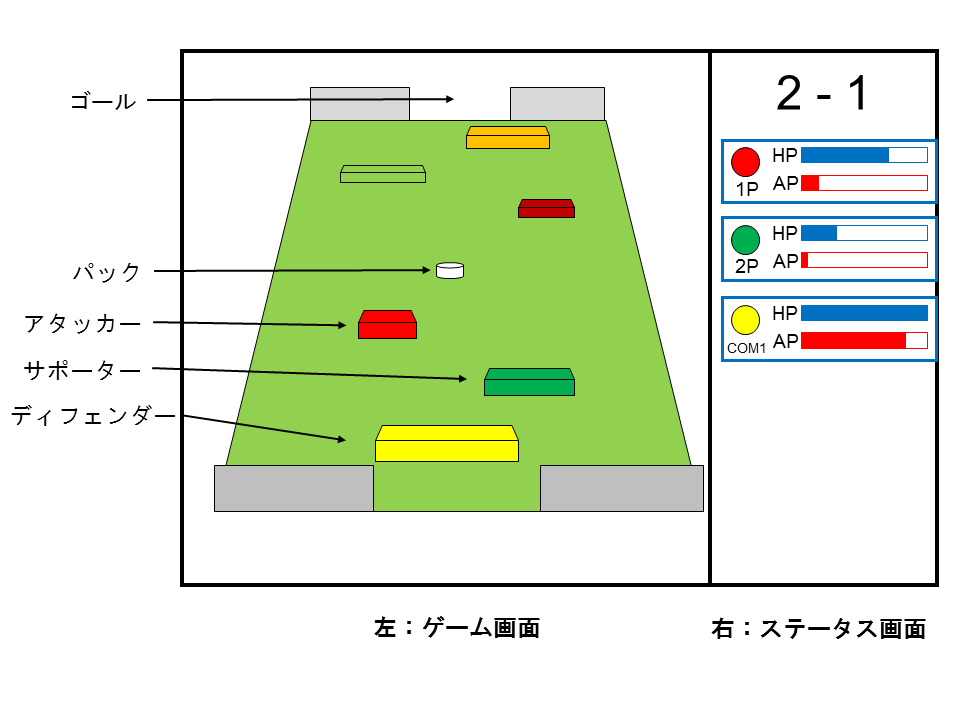
\includegraphics[scale=0.6]{kikaku.png}
    \caption{イメージ図}
    \label{fig:image}
  \end{center}
\end{figure}
%
\subsection{コンセプト}
コンセプトは「新感覚アクションゲーム」である.単なるホッケーゲームではなく,基本能力と必殺技を駆使して戦うという点が「新感覚」である.また,「分かりやすい操作」と「やっているうちに理解できるルール」を目標としている.\\
%
\subsection{各プレイヤーの説明}
\subsubsection{アタッカー(人間)}
アタッカーは,攻撃を得意とするプレイヤーである.

アタッカーが打ったパッドは速くなる.
%
\subsubsection{ディフェンダー(コンピュータ)}
ディフェンダーは,コンピュータが操作するプレイヤーでゴールを守る.また,アタッカーとサポーターの体力が0になったときに,身代わりになる.

ディフェンダーが打ったパッドは遅くなる.
%
\subsubsection{サポーター(人間)}
サポーターは,アタッカーとディフェンダーの体力回復をするプレイヤーである.サポーターが攻撃を受けると,ディフェンダーとアタッカーの体力が回復する.サポーターの体力は,時間が経つと回復する.
%
\subsection{ゲームの流れ}
各クライアントはサーバーに接続する.接続した順に1P,2P,3P,4Pとなる.「1Pと2P」「3Pと4P」がチームになる.各プレイヤーは「アタッカー」か「サポーター」を選択するが,もし被ってしまった場合はランダムに選択される.1Pはゲーム開始前に,「何点先取で勝ちにするか」などのルール設定をする.設定が終わると,カウントダウンと共にゲームが始まる.

各プレイヤーは左右方向に移動し,パッドを跳ね返す.ただ単に跳ね返すだけでなく,仲間と協力をしたり,必殺技を使うことで点数を取る.

点数を取ると,体力と必殺技ゲージはリセットされる.点数を取られた方からパッドを発射する.

開始前に設定した点数に達したほうが勝ちとなる.
%
\subsection{世界観}
\begin{boxnote}
みなさんは,サンタさんがクリスマス以外は何をして過ごしていると思いますか?長年にわたる調査の結果,僕たちはエアーホッケーをしていることを突き止めました.そのエアーホッケーは,普通の人間たちがプレイしているものとは全然違ったものでした.私達はサンタさんがプレイしている珍しいエアーホッケーをゲームで再現することにしました.最後に,皆さんに忠告があります.このゲームをクリスマスの日にプレイしないでください.エアーホッケーに熱中したサンタさんがプレゼントを届けることを忘れてしまいます.
\end{boxnote}
\section{構造体とモジュールの説明}
\subsection{構造体}
構造体PLAYER
\begin{table}[H]
  \begin{center}
    \begin{tabular}{|r||p{4em}|p{30em}|} \hline
      データ型 & 変数名 & 内容 \\ \hline
      int & type & プレイヤーの種類(0:アタッカー 1:サポーター 2:ディフェンダー)\\
        int & hp & プレイヤーの体力\\
        int & ap & 必殺技ポイント\\
        int & x & プレイヤーのX座標\\ \hline
    \end{tabular}
  \end{center}
\end{table}
構造体PAD
\begin{table}[H]
  \begin{center}
    \begin{tabular}{|r||p{4em}|p{30em}|} \hline
      データ型 & 変数名 & 内容 \\ \hline
      int & speed & パッドの速度\\
      int & x & パッドのX座標\\
      int & y & パッドのY座標\\ \hline
    \end{tabular}
  \end{center}
\end{table}
%
\subsection{モジュールの説明}
\begin{enumerate}
\item ネットワークモジュール \mbox{}\\
  サーバ・クライアント間の通信に関する処理を行う.
\item ゲーム処理モジュール \mbox{}\\
  ゲームパッドからの入力を受け取る・パッドの動きを計算する.
\item グラフィック・サウンドモジュール \mbox{}\\
  ゲーム画面・ステータス表示を描画する.また,BGMや効果音等の処理も行う.
\end{enumerate}

\subsection{各モジュールの外部関数}
\subsubsection{サーバー}
\begin{enumerate}
  \item ネットワークモジュール
    \begin{table}[H]
      \begin{center}
        \begin{tabular}{|c|p{3em}p{30em}|} \hline
          \multicolumn{3}{|l|}{{\tt void setup\_server(u\_short port)}}\\ \hline \hline
          機能 & \multicolumn{2}{|l|}{サーバーの初期設定を行う}\\
          引数 & port & ポート番号\\
          返り値 & なし & \\ \hline
        \end{tabular}
      \end{center}
    \end{table}
%
    \begin{table}[H]
      \begin{center}
        \begin{tabular}{|c|p{3em}p{30em}|} \hline
          \multicolumn{3}{|l|}{{\tt void recv\_data(int cid, void *data, int size)}}\\ \hline \hline
          機能 & \multicolumn{2}{|l|}{クライアントからデータを受信する}\\
          引数 & cid & クライアントID\\
          & data & 受信データ\\
          & size & 受信データのサイズ\\
          返り値 & なし & \\ \hline
        \end{tabular}
      \end{center}
    \end{table}
%
    \begin{table}[H]
      \begin{center}
        \begin{tabular}{|c|p{3em}p{30em}|} \hline
          \multicolumn{3}{|l|}{{\tt void recv\_data(int cid, void *data, int size)}}\\ \hline \hline
          機能 & \multicolumn{2}{|l|}{{\tt クライアントへデータを送信する}}\\
          引数 & cid & クライアントID\\
          & data & 送信データ\\
          & size & 送信データのサイズ\\
          返り値 & なし & \\ \hline
        \end{tabular}
      \end{center}
    \end{table}
%
    \begin{table}[H]
      \begin{center}
        \begin{tabular}{|c|p{3em}p{30em}|} \hline
          \multicolumn{3}{|l|}{{\tt void terminate\_server(void)}}\\ \hline \hline
          機能 & \multicolumn{2}{|l|}{クライアントとの接続を切断する}\\
          引数 & なし & \\
          返り値 & なし & \\ \hline
        \end{tabular}
      \end{center}
    \end{table}
%
\item ゲーム処理モジュール
      \begin{table}[H]
        \begin{center}
          \begin{tabular}{|c|p{3em}p{30em}|} \hline
            \multicolumn{3}{|l|}{{\tt void field\_set(void)}}\\ \hline \hline
            機能 & \multicolumn{2}{|l|}{受信したデータを元に,パッドの動きを計算する}\\
            引数 & なし & \\
            返り値 & なし & \\ \hline
          \end{tabular}
        \end{center}
      \end{table}
\end{enumerate}
%
\subsubsection{クライアント}
\begin{enumerate}
  \item ネットワークモジュール
      \begin{table}[H]
        \begin{center}
          \begin{tabular}{|c|p{6em}p{27em}|} \hline
            \multicolumn{3}{|l|}{{\tt void client\_server(char *server\_name, u\_short port)}}\\ \hline \hline
            機能 & \multicolumn{2}{|l|}{クライアントの初期設定を行う}\\
            引数 & server\_name & サーバのホスト名\\
            & port & ポート番号\\
            返り値 & なし & \\ \hline
          \end{tabular}
        \end{center}
      \end{table}
%
      \begin{table}[H]
        \begin{center}
          \begin{tabular}{|c|p{3em}p{30em}|} \hline
            \multicolumn{3}{|l|}{{\tt void recv\_data(void *data, int size)}}\\ \hline \hline
            機能 & \multicolumn{2}{|l|}{サーバからデータを受信する}\\
            引数 & data & 受信データ\\
            & size & 受信データのサイズ\\
            返り値 &なし & \\ \hline
          \end{tabular}
        \end{center}
      \end{table}
%
      \begin{table}[H]
        \begin{center}
          \begin{tabular}{|c|p{3em}p{30em}|} \hline
            \multicolumn{3}{|l|}{{\tt void recv\_data(void *data, int size)}} \\ \hline \hline
            機能 & \multicolumn{2}{|l|}{サーバへデータを送信する}\\
            引数 & data & 送信データ\\
            & size & 送信データのサイズ\\
            返り値 & なし & \\ \hline
          \end{tabular}
        \end{center}
      \end{table}
%
      \begin{table}[H]
        \begin{center}
          \begin{tabular}{|c|p{3em}p{30em}|} \hline
            \multicolumn{3}{|l|}{{\tt void terminate\_client(void)}}\\ \hline \hline
            機能 & \multicolumn{2}{|l|}{サーバとの接続を切断する}\\
            引数 & なし & \\
            返り値 & なし &\\ \hline
          \end{tabular}
        \end{center}
      \end{table}
%
\item ゲーム処理モジュール\\
      \begin{table}[H]
        \begin{center}
          \begin{tabular}{|c|p{3em}p{30em}|} \hline
            \multicolumn{3}{|l|}{{\tt void gamepad\_input(void)}}\\ \hline \hline
            機能 & \multicolumn{2}{|l|}{ゲームパッドの入力を受け取る}\\
            引数 & なし & \\
            返り値 & なし & \\ \hline
          \end{tabular}
        \end{center}
      \end{table}
%
\item グラフィック・サウンドモジュール\\
      \begin{table}[H]
        \begin{center}
          \begin{tabular}{|c|p{3em}p{30em}|} \hline
            \multicolumn{3}{|l|}{{\tt void draw\_field(void)}}\\ \hline \hline
            機能 & \multicolumn{2}{|l|}{ゲーム画面を描画する}\\
            引数 & なし & \\
            返り値 & なし & \\ \hline
          \end{tabular}
        \end{center}
      \end{table}
%
      \begin{table}[H]
        \begin{center}
          \begin{tabular}{|c|p{3em}p{30em}|} \hline
            \multicolumn{3}{|l|}{{\tt void draw\_status(void)}}\\ \hline \hline
            機能 & \multicolumn{2}{|l|}{ゲームのステータスを描画する}\\
            引数 & なし & \\
            返り値 & なし & \\ \hline
          \end{tabular}
        \end{center}
      \end{table}
\end{enumerate}

\section{各々の担当}
\begin{table}[H]
  \begin{tabular}{ll}
    木村 & ネットワーク担当\\
    好川 & グラフィック担当\\
    長滝谷・近藤 & ゲーム担当\\
  \end{tabular}
\end{table}
\section{ガントチャート}
\begin{figure}[H]
  \begin{center}
    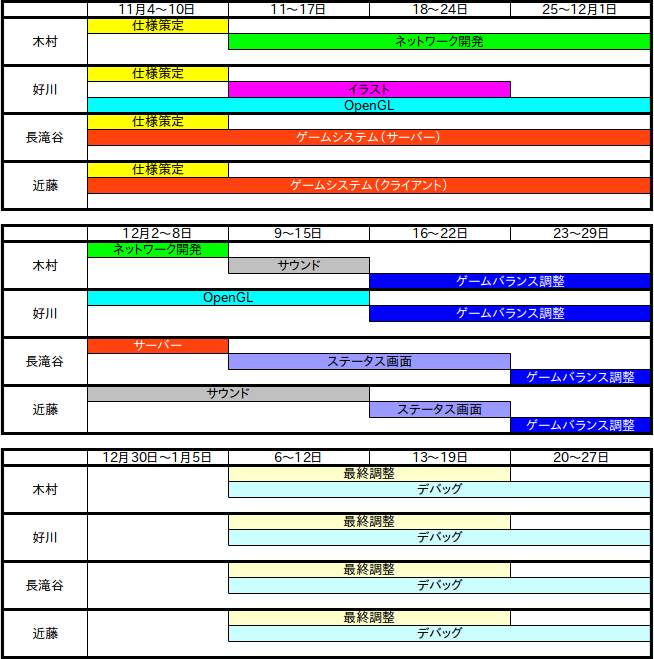
\includegraphics[scale=0.5]{chart.png}
  \end{center}
\end{figure}
\end{document}
